\graphicspath{{chapters/images/05/}}
\chapter{Mapping}

\section{Introduction}
Mapping and assembly are the operations that allow us to understand sequencing data producing assemblies.

\begin{multicols}{2}
    \begin{itemize}
        \item \textbf{Mapping} is a key step in a modern genomic analysis and consists in the process of aligning the reads on a reference genome in order to assign them to a specific location.
            Insights like the expression level of genes can be gained.
        \item \textbf{Assembly} is the process of aligning and merging overlapping sequences in longer consensus sequences in order to reconstruct the original sequence or genome.
    \end{itemize}
\end{multicols}

A consensus sequence is the calculated order of most frequent residues, either nucleotide or amino acid, found at each position in a sequence alignment.
In many cases, someone may have already assembled the genome or part of the genome (available reference sequences), so sequence assembly is not needed.
Assembly will be needed however when studying new organisms.
Mapping and assembly need to solve some problem related to the sequencing data:

\begin{multicols}{2}
    \begin{itemize}
        \item absence of DNA fragments covering the gaps, makes it difficult to order the contigs (since there is no connection)
        \item presence of DNA artefacts (those must be discriminated with Quality Control)
        \item repeated sequences
    \end{itemize}
\end{multicols}

    \subsection{Coverage}
    The coverage, or read depth, is the average number of reads representing a given nucleotide in the reconstructed sequence.
    The coverage of a genome is defined as the average coverage of each single nucleotide across all nucleotides of the genome.
    The coverage can be represented with a coverage map and can also be defined theoretically as:

    $$Cov = \frac{N\cdot L}{G}\sim\ln \frac{G}{L\cdot\varepsilon}$$

    Where $G$ is the length of the genome, $N$ is the  number of reads, $L$ is the average read length and $1-\varepsilon$ is the probability to cover the entire genome with coverage $Cov$.
    More reads obtained during sequencing the higher the coverage.
    In particular, the number $N$ of reads needed to cover the entire genome with probability $1-\varepsilon$ is:

    $$N\sim\frac{G}{L}\ln\frac{G}{L\cdot\varepsilon}$$

    \subsection{Mapping process}
    In general, the sequence mapping process consists in performing comparisons between experimental sequence data with some reference information.
    The comparison can lead to obtaining new information, such as the presence of SNPs which can be linked to pathological conditions for example.

    \begin{figure}[h]
    \centering
    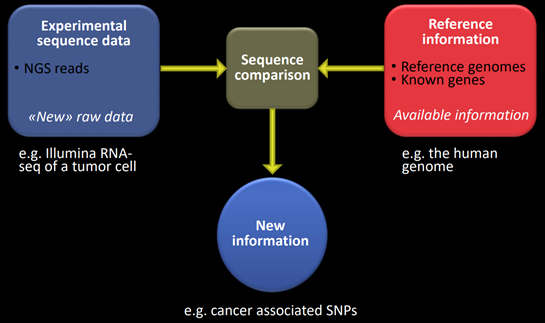
\includegraphics[width=0.6\textwidth]{SequenceComparison.png}
    \caption{}
    \end{figure}

\section{Mapping algorithms}
Over time many different mapping algorithms were implemented.
Ideally, the simplest aligning algorithm could consists in: a complete search: starting from the first position on the reference, the query sequence is controlled against it and the correct nucleotides are counted and summed forming a score.
This is repeated for all positions until a perfect match is found or the position with the highest score is taken.
This algorithm is very naive and does not take into account insertions and deletions.

    \subsection{Local vs Global alignment}
    Sequence alignment can follow two different approaches.

    \begin{multicols}{2}
        \begin{enumerate}
            \item In global alignment an attempt is made to align completely the $2$ sequences.
                It is referred as end to end alignment.
                It finds the best alignment across the whole two sequences.
                This approach is suitable for comparing closely related sequences like homologous genes.
            \item Local alignment, on the other hand, focuses on finding regions of similarity in parts of the sequences.
                It aligns subsequences of the query sequence to a subsequence of the target sequence.
                This approach is suitable for aligning more divergent sequences or distantly related sequences.
                It is used for example for finding out conserved patterns in DNA sequences of motifs in two proteins.
        \end{enumerate}
    \end{multicols}

    Sequence similarity is connected with evolutionary distance.
    Very high similarity implies a very low distance.
    But when the similarity goes down and reaches the twilight zone as in \ref{evodist} it is more difficult to define the evolutionary distance and to give meaning to results.

    \begin{figure}[h]
        \centering
        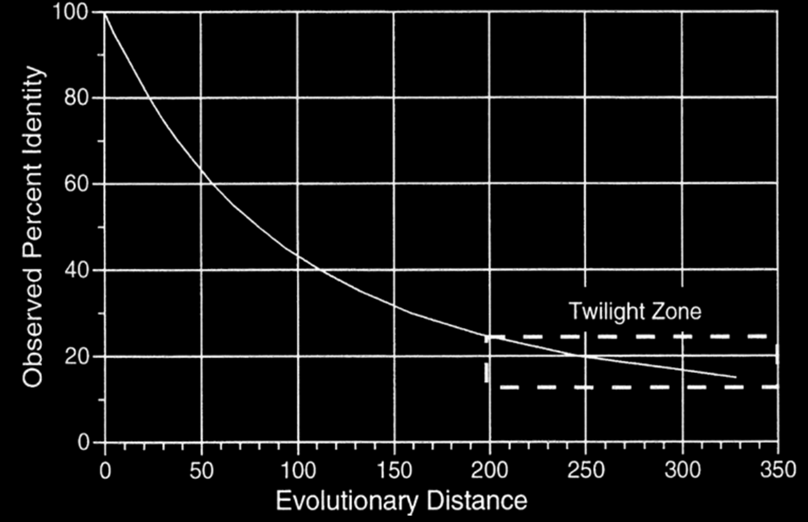
\includegraphics[width=0.6\textwidth]{EvolutionaryDistance.png}
        \caption{}
        \label{evodist}
    \end{figure}

    \subsection{Smith-Waterman algorithm}
    The Smith-Waterman algorithm is a local-alignment algorithm based on dynamic programming, whose aim is to find the best match among all possible optimal local alignment with respect to the scoring system used.
    Consider two molecular sequences $A = a_1a_2\dots a_n$ and $B = b_1b_2\dots b_m$.
    Given a similarity $s(a,b)$ of elements of the sequence and $W_k$ the weight of deletions of length $k$, to find pairs of segments with high degrees of similarity, a matrix $H$ is set up such that:

    $$H_{k0} = H_{0l} = 0\qquad \forall 0\le k\le n\land 0\le l\le m$$

    $H_{ij}$ si the maximum similarity of two segments ending in $a_i$ and $b_j$.
    $H_{ij}$ is computed such that:

    $$H_{ij} = \max(H_{i-1, j-1} + s(a_i, b_j), \max\limits_{k\ge 1}(H_{i-k, j}-W_k), \max\limits_{l\ge 1}(H_{i, j-l}-W_k), 0)$$

    With $1\le i\le n$ and $1\le j\le m$.
    So $H_{ij}$ is:

    \begin{multicols}{2}
      \begin{itemize}
        \item $H_{i-1, j-1} + s(a_i, b_j)$ If $a_i$ and $b_j$ are associated.
        \item $H_{i-k, j}-w_k$ if $a_i$ is at the end of a deletion of length $k$.
        \item $H_{i-k, j}-W_l$ if $b_j$ is at the end of a deletion of length $l$.
        \item $0$ is used to prevent calculated negative similarity, indicating no similarity up to $a_i$ and $b_j$.
      \end{itemize}
    \end{multicols}

    The pair of segments with maximum similarity is found first by locating the maximum element of $H$.
    The other elements are determined sequentially with a traceback procedure ending with an element of $H$ equal to $0$.
    This procedure other than identifying the elements produces their alignment.
    The parameters  where:

    $$s(a_i, b_j) = \begin{cases} 5 & a_i = b_j \\ -3 & a_i\neq b_j\end{cases}$$

    And

    $$W_k = \frac{1}{3}k$$

    This algorithm in particular allows for the alignment of sequences that contained both mismatches and internal deletions.

    \subsection{Needleman-Wunsch algorithm}
    This global alignment algorithm was developed in 1970 and is also based on dynamic programming.
    The purpose of the algorithm is to find all possible alignments having the highest score.
    The idea is the same of the Smith-Waterman, but it has difference in initialization and computing of the matrix element, in particular:

    $$H_{00} = 0$$

    $$H_{ij} = \max(H_{i-1, j-1} + \alpha s(A_j, B_i), H_{i-i, j} + d, H_{i,j-1} + d)$$

    Again a scoring function $s$ needs to be defined.
    The fact that the max function contains no 0 anymore means that we are always comparing with the first nucleotide of the sequence.

    \subsection{Heuristic methods}
    New algorithms were implemented later.
    BWA and BowTie2 are the best ones available right now for short reads.
    Blast could also work too but it would take too much time.

    \begin{figure}[h]
    \centering
    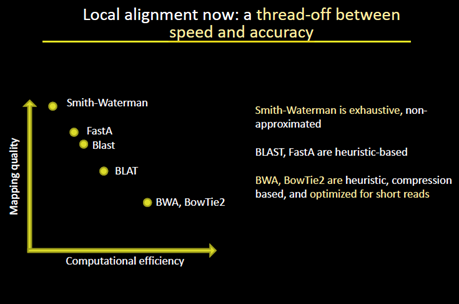
\includegraphics[width=0.6\textwidth]{LocalAlignment.png}
    \caption{}
    \end{figure}

    This new algorithms are based on heuristic methods: the solution found is not the optimal, but it is the best approximation given some constrains.
    An heuristic is any approach to problem solving or self-discovery that employs a practical method that is not guaranteed to be optimal, perfect, or rational, but is nevertheless sufficient for reaching an immediate, short-term goal or approximation.
    Where finding an optimal solution is impossible or impractical, heuristic methods can be used to speed up the process of finding a satisfactory solution.
    For example BLAST return an alignment on a fixed level of similarity and no result under that level of quality.
    BWA and BowTie2 are also compression based algorithms: they exploit data compression techniques in order to compress reference genome files to reduce the number of bits used to encode it.

    \subsection{BLAST (Basic Local Alignment Search Tool)}
    Despite its limitations, Blast is still widely used due to is low computational power.
    The Blast algorithm involves three steps:

    \begin{multicols}{2}
        \begin{enumerate}
            \item Seeding: find perfect or almost exact k-mer matches.
                The idea is to look for identical short matches and try to expand from that.
            \item Extension: extend the seeds at point one $1$ with possibly some non-exact but high-score matches, that permit to obtain better alignments.
            \item Evaluation: create alignments for the regions of high-scoring extended seeds.
                Every time the statistical significance of the match is evaluated with methods inspired on the NW and SW approaches.
        \end{enumerate}
    \end{multicols}

    If a k-mer length does not result in any matches its length can be decreased, increasing the computation time needed.

        \subsubsection{Blast flavours}
        Blast comes in many flavours, depending on what is the desired output and input:

        \begin{multicols}{2}
            \begin{itemize}
                \item Blastp: compares an amino acid query sequence against a protein sequence database.
                \item Blastn: compares a nucleotide query sequence against a nucleotide sequence database.
                \item Blastx: compares a nucleotide query sequence translated in all reading frames against a protein sequence database.
                    This can be done to find potential translation products of unknown nucleotide sequences.
                \item Tblastn: compares a protein query sequence against a nucleotide sequence database dynamically translating in all reading frames.
                \item Tblastx: compares the six-frame translation of a nucleotide query sequence against the six-frame translation of a nucleotide sequence database.
            \end{itemize}
        \end{multicols}

        \subsubsection{Scoring matrices}
        Scoring matrices are the way in which blast score matches and mismatches.
        They are very important especially for amino acids and they are used to score alignments between protein sequences.
        Blosum 62 (BLOcks SUbstitution Matrix) is one of the most used.
        Non simple penalties in substitutions of different amino acids are used, based on the functional properties of the substitutions.
        A scoring matrix contains values proportional to the probability that amino acid $i$ mutates into amino acid $j$ for all pairs of amino acids.
        Such matrices are constructed by assembling a large and diverse sample of verified pairwise alignments of protein sequences.

        \subsubsection{Blast parameters}
        Other parameters can be set in BLAST:

        \begin{multicols}{2}
            \begin{itemize}
                \item Max target sequences: number of reported sequences.
                \item Expected threshold: e-value.
                \item Words size: seed length.
                \item Gap cost: cost for adding multiple gaps.
                    It can be linear or non linear.
                \item Filter low complexity regions to avoid getting stuck.
            \end{itemize}
        \end{multicols}

        \subsubsection{BLAST E-value}
        The \emph{e-value} represents the number of distinct alignments with a score equivalent to or higher than $S$, that are expected to occur in a database search by chance.
        It is computed as:

        $$Evalue = Kmne^{-\lambda S}$$

        Where $K$ and $\lambda$ depend on the substitution matrix and on gab penalties, $n$ is the query length, $m$ is the length of the sequences of the database and $S$ is the matching score.
        An e-value of $10$ means that up to $10$ alignments can be expected to be found just by chance, given the same size of a random database.
        E-value can be used as a first quality filter for the BLAST search result, to obtain only results equal to or better than the number given by the e-value option.
        Blast results are sorted by E-value by default (best hit in first line).
        The smaller the e-value, the better is the match.
        A small e-value means a low number of hits of high quality, whereas a high e-value indicates many hits, partly of low quality.
        There is a relationship between the E-value and the p-value.

        \begin{multicols}{2}
            \begin{itemize}
                \item The E-value is the number of sequences that we would find by chance;
                \item The p-value measures the probability of finding by chance another sequence with an equal or better score.
            \end{itemize}
        \end{multicols}

        In particular:

        $$Pval = K e^{-\lambda S} = Evalue/mn$$

    \subsection{Speed seed alignment}
    There are algorithms implemented 10/15 years ago that focus on seeds and are note used any more.
    Those methods cut both the reads and the reference sequence into small seeds.
    The reference seeds are then stored in an hash look-up table.
    The idea is to do that for all possible k-mers of the two sequences.
    Algorithms based on this approach are: Maq, SOAP, MOSAIK.
    This present problems in the presence of SNPs:

    \begin{multicols}{2}
        \begin{itemize}
            \item 1 SNPs means that at most 1 seed is not-matching.
            \item $X$ SNPs means that at most $X$ seeds are not-matching.
        \end{itemize}
    \end{multicols}

    The problem of these algorithms is that the lookup table is too big to be fully loaded in memory.

    \subsection{Burrow-Wheeler alignment}
    The Burrows-Wheeler algorithm is used in BowTie and Bowtie2.
    The Borrow-Wheeler algorithm is based on a very efficient way to store the reference genome, based on the BW transformation, that allows to have a reference hash table much smaller than the one of the speed seed approach.
    This particular method is successful because the compression is reversible and so the reference does not need to be decompressed.
    It is this reversible property in fact that guarantees that the reads can be found in the genome.
    The search is based on finding suffixes of the reads in the BW structure.
    With this approach the index of the human genome is around 2GB.
    The BW-based algorithms are the fastest currently available.

        \subsubsection{Reversibility of the Borrow-Wheeler compression}
        To compress a word:

        \begin{multicols}{2}
            \begin{enumerate}
                \item Add a terminator to the word.
                \item Form a matrix containing all the rotations of the word as rows.
                \item Sort them based on lexicographic order.
                \item Take the last column.
            \end{enumerate}
        \end{multicols}

        In the end this string is much more compressible because the same letters tend to be grouped together.
        In order to reverse the transformation

        \begin{multicols}{2}
            \begin{enumerate}
                \item Repeat until the matrix is square:
                    \begin{enumerate}
                        \item the input sequence result of the compression is added as a column to a matrix.
                        \item Sort the rows of the matrix according to lexicographical order.
                    \end{enumerate}
                \item The row where the last element is the terminator is the untransformed input.
            \end{enumerate}
        \end{multicols}

        This reverse transformation can be made faster through the last-first property.

        \subsubsection{LF (Last-First) property}
        The LF property is then applied to the matrix of all rotations to get back the input sequence.
        This is possible because the $ith$ occurrence of character $X$ in the last column corresponds to the same text character as the $ith$ occurrence of $X$ in the first column.
        Following this property the word is reconstructed backward:

        \begin{multicols}{2}
            \begin{enumerate}
                \item Look the first element $c$ of the last column and add it to the end of the output.
                \item Go to the corresponding $ith$ occurrence of $c$ in row $j$.
                \item Add to the output element in the last column in row $j$.
                \item Repeat with $c = MAT_{j,last}$ until the terminator is found.
            \end{enumerate}
        \end{multicols}

        \subsubsection{Exact mapping using LF property}
        When performing a mapping operation sequence matching can be done using the compressed database.
        Backward exact mapping works by calculating the range of matrix rows beginning with successively longer suffixes of the query.
        Doing the backward matching we exploit the characteristics of the BWT transform.
        This same approach could be used to find a match between a query read and a reference genome which has been compressed using the BW alignment.
        The problem is that it does not take into accounts indels or mismatches.

        \subsubsection{Inexact mapping}
        A possible solution to this problem could be the inexact mapping.
        Perform exact mapping and, if the query is not found, go back and perform backtracking by hypothesising mismatches.
